\documentclass{beamer}
\usetheme{Madrid}

\usepackage[francais]{babel}
\usepackage{amsmath}

\title{Une octave dissonante}
\author{Henry Dumant - Simon Vic} 
\centering
\date{Mai 2020}

\newcommand{\f}{\frac}
\DeclareMathOperator{\e}{e}

\begin{document}
\maketitle


\begin{frame}{Introduction}
\framesubtitle{Phénomène de battements}

\begin{itemize}
    \item Addition de deux signaux de fréquences proches
    $$ \cos(f x) + \cos((f + \varepsilon)x) = 2 \cos((f + \frac{\varepsilon}{2})x) \cos(\frac{\varepsilon}{2}) $$
    \begin{center}
        \includegraphics[scale = 0.4]{battements.png}
    \end{center}
    \item Entraine une dissonance : modulation de l'amplitude à une fréquence beaucoup plus petite.
    
\end{itemize}
\end{frame}

\begin{frame}{Introduction}
\framesubtitle{Quasi-octave dissonante \footnote{Tuning Timbre Spectrum Scale (2004)}}
\begin{itemize}
    \item En musique, on entend parfois des dissonances \emph{au quasi-octave près} (c'est-à-dire pour une fréquence proche du double de la note), pourquoi ?

    \item Instruments de musique dits \emph{harmoniques} : les notes jouées sont la superposition de plusieurs ondes de fréquences multiples de la fréquence \emph{fondamentale}, les \emph{harmoniques}.
    \item Ce sont ces harmoniques qui dissonent.
\end{itemize}
\end{frame}

\begin{frame}{Introduction}
\framesubtitle{Quasi-octave dissonante, exemple}
\begin{itemize}
\item
    Alice joue un \textbf{la} 440 au saxophone, elle emet en fait : 
    $$ alice(t) = a_1 \cos(440t) + a_2 \cos(880t) + a_3 \cos(1320t) + \dots $$
    \item Arthur veut jouer un \textbf{la} 880 (octave au dessus) mais il joue un peu trop haut... 881 Hz :
    $$ arthur(t) = b_1 \cos(881t) + b_2 \cos(1762t) + \dots $$
    \item La deuxième harmonique d'Alice (880Hz), et le fondamental d'Arthur (881Hz) dissonent, ainsi que la quatrième harmonique d'Alice (1760) et la deuxième d'Arthur (1762), etc.
    
\end{itemize}
\end{frame}

\begin{frame}{Introduction}
\framesubtitle{Des instruments non-harmoniques}

\begin{itemize}
    \item \emph{Instruments non-harmonique} : les fréquences propres ne sont pas multiples d'une fréquence fondamentale.
    \item Il en existe en \og vrai \fg{}, comme le gamelan :
    \begin{center}
        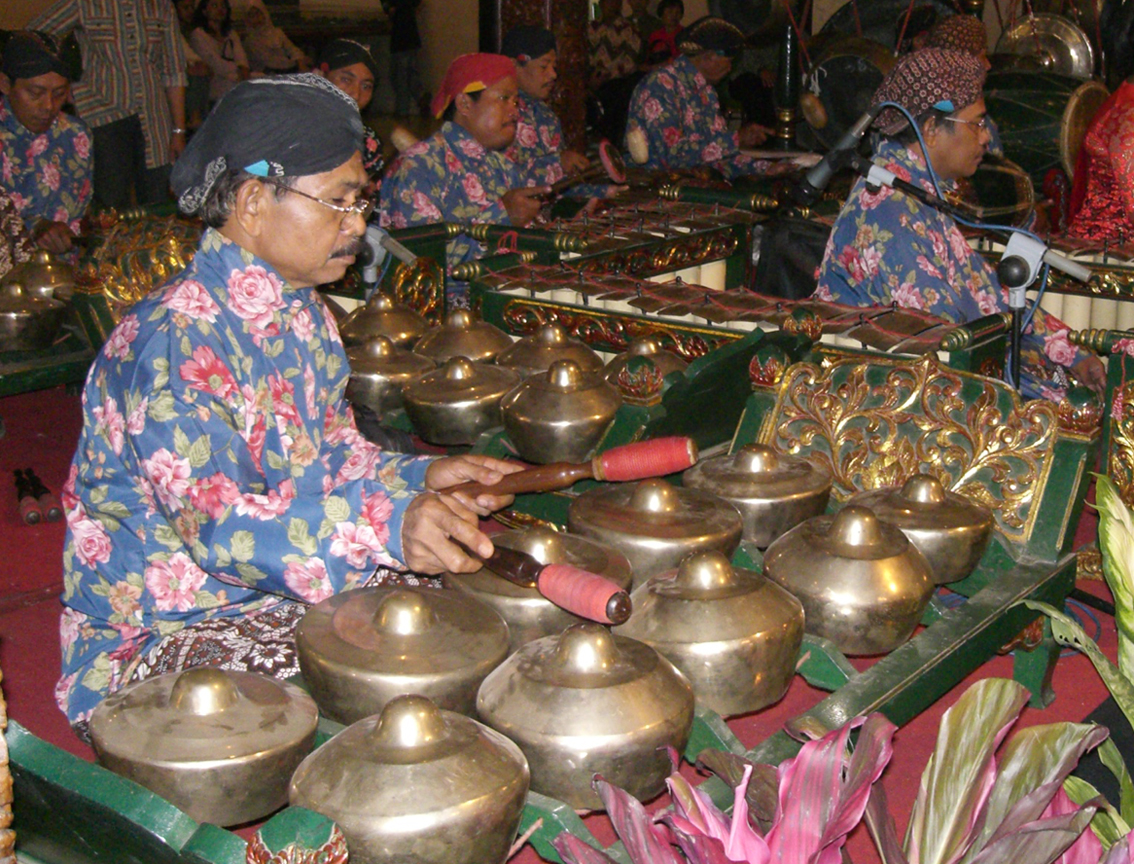
\includegraphics[scale = 0.5]{gamelan.jpeg}
    \end{center}
    \item On peut en construire numériquement, ou essayer de chercher une forme géométrique qui vibre à un spectre donné : c'est l'objectif de ce stage...
\end{itemize}
    
\end{frame}

\begin{frame}{Introduction}
\framesubtitle{Objectif du stage}

\begin{itemize}
    \item Trouver une forme géométrique qui produit un son de la forme :
    $$ s_f(t) = a_1 \cos(ft) + a_2 \cos((2+\varepsilon)ft) + a_3 \cos((3+\varepsilon)ft) + \dots $$
    pour une fréquence fondamentale de $f$.
    \item De sorte que $s_f$ et l'octave supérieur parfait  $s_{2f}$ dissonent.
    
\end{itemize}
\end{frame}


\begin{frame}{Introduction}
\framesubtitle{Problème physique}
\begin{itemize}
    \item On s'intéresse à l'équation des ondes :


\begin{block}{Équation des ondes}
$$ \Delta u = \f{1}{c^2} \frac{\partial^2 u}{\partial t^2}   $$
\end{block}

sur un domaine $\Omega$

\item On cherche à résoudre cette EDP à partir d'une base $(\varphi_n)_n$ hilbetienne de $\mathbf{L}^2(\Omega)$, de vecteurs propres de l'opérateur linéaire laplacien.

\item Le problème est donc un problème d'algèbre linéaire, que l'on simplifie à un problème en dimension finie.

\end{itemize}

\end{frame}

\begin{frame}{Le problème direct}
  \framesubtitle{Problème continu}

\begin{itemize}
       \item Déterminer le spectre de vibration d'une forme géométrique (dimension 1,2 et 3)
        \item $\Omega$ (surface régulière) = objet
        \item $\Delta_\Omega$ = opérateur de Laplace-Beltrami  							          		    \item $\phi$ = amplitude de la vibration
        
\end{itemize}
\begin{block}{Equation de vibration de la surface}
\[-\Delta_\Omega\phi=\frac{\lambda}{c^2}\phi \]
\end{block}

\begin{itemize}
        \item $\sqrt{\lambda}$ = fréquence du son résultant
\end{itemize}
   
\end{frame}

\begin{frame}{Le problème direct}
  \framesubtitle{Discrétisation du problème}

\begin{itemize}
       \item Utilisation du langage des graphes
        \item $B\in\mathcal{M}_{n,m}(\mathbb{R})$ = matrice d'incidence du graphe du maillage initial
       \item Maillage de $\Omega$ = graphe pondéré orienté
       \item $W_\Omega\in\mathcal{M}_{n,n}(\mathbb{R})$ = matrice des poids des arrêtes du graphe = forme, rigidité de l'objet physique ($\Omega$)
       \item $\Delta_\Omega \longleftrightarrow -B^TW_\Omega B$
       
\end{itemize}
\begin{block}{Problème discrétisé}
\[\mbox{Eléments propres de } B^TW_\Omega B ?\]
\end{block}

\begin{itemize}
        \item Problème de dimension infinie ramené à un problème d'algèbre linéaire de dimension finie. 
\end{itemize}

\end{frame}

\begin{frame}{Le problème direct}
  \framesubtitle{Le cas d'une corde fixée aux extrémités}

\includegraphics[scale=0.5]{graphe.png}  
$
B = \begin{pmatrix}
    -1 & 1 &  & (0) \\ 
    & \ddots & \ddots  \\ 
    (0) & & -1 & 1
\end{pmatrix}
$\\

$W_\Omega = \mbox{diag}(\infty,1,1,...,1,1,\infty)$\\

\end{frame}

\begin{frame}{Le problème direct}
  \framesubtitle{Modes de vibration}

\includegraphics[scale=0.5]{first_partials_1d.png}  

\end{frame}

\begin{frame}{Le problème direct}
  \framesubtitle{Le cas d'une corde fixée aux extrémités : lien harmoniques et fondamental}
  
  On a démontré que si le nombre de points $N$ de la discrétisation est grand et $k$ est petit devant $N$ alors on a l'estimation suivante pour le $k$-ième partiel: $\mu_k=\sqrt{\frac{\lambda_k}{\lambda_1}}\simeq k$. \\
  
\includegraphics[height=3cm]{Capture d’écran 2020-05-11 à 18.54.34.png}  
  
\end{frame}

\begin{frame}{Le problème direct}
  \framesubtitle{Une forme quelconque en deux dimensions : un disque}
  
 \begin{center}
     \includegraphics[scale = 0.7]{peau_ronde_dirichlet.png}
 \end{center}

  
\end{frame}

\begin{frame}{Piste pour le problème inverse}
  
\begin{itemize}
       \item Déterminer une forme d'objet qui donne un spectre de vibration donné
        \item $\Sigma\in\mathbb{R}^m$ = spectre de fréquences donné
        \item $W_\Omega$ = inconnue du problème
\end{itemize}

\begin{block}{Equation du problème}
\[\mbox{Sp}(B^TW_\Omega B)=\Sigma\]
\end{block}

\begin{itemize}
       \item Minimisation de $E(W)=\Vert \mbox{Sp}(B^TW_\Omega B)-\Sigma\Vert^2$. \footnote{Computational design of metallophone contact sounds (Bharaj et al. 2015) ; Izospectralization, or how to hear a shape, style, and correspondence (2019)}
        \item Problème : telle qu'est implémentée np.eigs, il est difficile de minimiser $E$, il va donc falloir chercher une (des) nouvelle(s) manière(s) d'implémenter une fonction qui calcule(nt) les valeurs propres et les vecteurs propres d'une matrice.
\end{itemize}

\end{frame}



\end{document}
